%!TEX root = ../thesis.tex
%*******************************************************************************
%****************************** Second Chapter *********************************
%*******************************************************************************



\chapter{Theory framework}

\graphicspath{{1_MainChapters/Chap2_Theory/Figs}}

This chapter provides an overview of the theoretical framework that underpins the research presented in this thesis.
The chapter begins with a discussion of the Standard Model of particle physics.
The chapter then introduces one possible extension to the Standard Model. To relate the theory to the experiments 
conducted at the Large Hadron Collider (LHC), the chapter concludes with a brief discussion of the modelling of proton-proton
collisions. This chapter is based on review articles of the Standard Model and particle physics~\cite{RevModPhys.71.S96,ParticleDataGroup:2022pth},
and the articles on the Randall-Sundrum model and phenomenology~\cite{Graviton_theory,Fitzpatrick:2007qr,Davoudiasl_2001}.

\section{The Standard Model of particle physics}
    The Standard Model of particle physics (SM) is a quantum field theory 
    describing the interactions of matter through three of the four 
    fundamental forces in nature: electromagnetic, weak, and strong 
    forces. Formulated from theoretical arguments and experimental 
    evidence, it is one of the most rigorously tested theories in physics. 
    Its core principle is the local gauge symmetry of the gauge group 
    $SU(3)_c \times SU(2)_L \times U(1)$. Here, the non-Abelian 
    $SU(3)_c$ and $SU(2)_L \times U(1)$ groups represent quantum chromodynamics (QCD) 
    and the electroweak sector, respectively.

    Figure~\ref{fig:SM_particles} summarise the particles
    in the Standard Model. Elementary particles in the model fall into two categories based on 
    their spin values: fermions, which have half-integer spin, and bosons, 
    which possess integer spin. The fundamental forces arise from interactions 
    between their corresponding gauge (spin-1) bosons and a subset of fermions. 
    Fermions and bosons are grouped in tables summarising their spin, 
    electric charge, and mass.

    Fermions are further classified into two basic types: leptons and quarks. 
    Each group has six particles, arranged into three generations. Every 
    fermion has an associated antiparticle with identical mass but opposite 
    quantum numbers. Leptons include the electron $(e)$, muon $(\mu)$, and tau $(\tau)$, 
    each paired with a corresponding neutrino $(\nu)$. Electrons, muons, 
    and taus are charged and progressively increase in mass, while neutrinos 
    are neutral and have very small masses. Quarks consist of up $(u)$, down $(d)$, 
    strange $(s)$, charm $(c)$, bottom $(b)$, and top $(t)$. They all possess 
    mass and are electrically charged, increasing in mass with each generation. 
    Additionally, quarks contain a colour charge, which determines their interaction 
    through the strong force.

    All fermions interact through the weak interaction, charged fermions engage 
    in electromagnetic interactions, and only quarks experience strong interactions. 
    The corresponding gauge bosons mediating these forces include the photon $(\gamma)$ 
    for the electromagnetic force, gluon $(g)$ for the strong force, and $W^+$, $W^-$, 
    and $Z$ bosons for the weak interaction. The theory also includes a scalar (spin-0) 
    boson, the Higgs boson $(H)$, which provides mass to both bosons and fermions 
    through the mechanism of spontaneous symmetry breaking within the electroweak 
    interaction. The discovery of the Higgs boson stands as a significant confirmation 
    of the predictive power of the SM. 

    \begin{figure}[htbp]
        \centering
        \includegraphics[width=1.0\textwidth]{Raster/SM_particles}
        \caption{
            The particles in the Standard Model of Particle Physics, with mass, charge, and spin. Taken from~\cite{quanta-magazine-2020}.
        }
        \label{fig:SM_particles}
    \end{figure}

    However, the Standard Model remains incomplete as it does not encompass gravity, 
    the fourth and weakest fundamental force, nor does it explain the observed 
    matter-antimatter asymmetry or the indirect evidence of dark matter. Therefore, 
    measuring Standard Model processes is crucial to uncovering discrepancies 
    between theory and experiment that could address these outstanding issues.

    In the following sections, we will discuss the symmetry principles,
    quantum field theory, the Standard Model of Particle Physics, and the gravitational extension.
    
    \subsection{Symmetry principles}
        The concept of symmetry is fundamental to the Standard Model. 
        According to the principle of Lorentz symmetry, the laws of 
        physics remain consistent for observers in different inertial reference 
        frames. This concept, along with quantum mechanics, bridges the gap between 
        classical mechanics and quantum field theories, which is essential for 
        understanding the Standard Model of particle physics.
        \subsubsection{Lagrangian formulation}
            In classical mechanics, the Lagrangian is a function of the
            generalised coordinates $q_i(t)$, generalised velocities $\dot{q}_i(t) = \frac{\text{d}q_i}{\text{d}t}$,
            and time $t$
            \begin{equation}
                L(q_i, \dot{q}_i) = T(q_i, \dot{q}_i) - V(q_i).
            \end{equation}
            where $T$ is the kinetic energy, and $V$ is the potential energy of the system.
            The action $S$ is defined as the integral of the 
            Lagrangian over time
            \begin{equation}
                S = \int L(q_i, \dot{q}_i) dt.
            \end{equation}
            The principle of least action states that the action $S$ is minimised
            along the path of motion of the system.
            A small perturbation, $q_i(t) \rightarrow q_i(t) + \delta q_i(t)$, should leave the action unchanged.
            The change in the action \( \delta S \) under the perturbation can be expressed as:
            \begin{equation}
                \delta S = 0 = \int_{t_1}^{t_2} \left( \delta q_i \frac{\partial L}{\partial q_i} + \delta \dot{q_i} \frac{\partial L}{\partial \dot{q_i}} \right) dt.
            \end{equation}
            This can be rearranged using integration by parts:
            \begin{equation}
                \delta S = 0 = \int_{t_1}^{t_2} \left( \delta q_i \frac{\partial L}{\partial q_i} + \frac{d}{dt} \left( \delta q_i \frac{\partial L}{\partial \dot{q_i}} \right) - \delta q_i \frac{d}{dt} \left( \frac{\partial L}{\partial \dot{q_i}} \right) \right) dt.
            \end{equation}
            By choosing the perturbation to vanish at the endpoints, the second term vanishes, and the equation simplifies to
            \begin{equation}
                \frac{\partial L}{\partial q_i} = \frac{d}{dt} \left( \frac{\partial L}{\partial \dot{q_i}} \right).
            \end{equation}
            This is the Euler-Lagrange equation, which describes the motion of the system.
        

            In field theories, the Lagrangian density, $L[\phi(x), \partial_{\mu}\phi(x)]$, is used instead of the $L$. 
            Here, $\phi(x)$ represents a scalar field dependent on the space-time four-vector $x$, 
            and $\partial_{\mu}\phi(x)$ is the derivative of the field with respect to the space-time coordinates
            \begin{equation}
                \partial_{\mu}\phi(x) = \frac{\partial \phi(x)}{\partial x^{\mu}}.
            \end{equation}
            The Lagrangian, as discussed in the previous paragraph, can be obtained by integrating the Lagrangian density over the space volume:
            \begin{equation}
                L = \int \mathcal{L}[\phi(x), \partial_{\mu}\phi(x)] d^{3}x.
            \end{equation}
            Additionally, the action S is defined by integrating the Lagrangian density over the entire four-dimensional spacetime:
            \begin{equation}
            S = \int \mathcal{L}[\phi(x), \partial_{\mu}\phi(x)] , d^{4}x.
            \end{equation}
            Similar to the classical mechanics, the Euler-Lagrange equation for the field $\phi(x)$ can be written as:
            \begin{equation}
                \partial_{\mu}(\frac{\partial \mathcal{L}}{\partial(\partial_\mu \phi)}) - \frac{\partial \mathcal{L}}{\partial \phi} = 0,
            \end{equation}
            following the same principle of least action. 
            Consider a free particle with mass $m$, the Lagrangian density can be written as:
            \begin{equation}
                \mathcal{L} = \frac{1}{2} \partial_{\mu}\phi(x) \partial^{\mu}\phi(x) - \frac{1}{2} m^{2} \phi^{2}(x).
            \end{equation}
            Using the Euler-Lagrange equation, the Klein-Gordon equation can be derived:
            \begin{equation}
                (\partial_{\mu}\partial^{\mu} + m^{2})\phi(x) = 0,
            \end{equation}
            which describes the motion of a free scalar field.
        \subsubsection{Symmetry and conservation Laws}
            Conservation laws are a direct consequence of the symmetry of the Lagrangian,
            not only in field theories but also in classical field theory and even in 
            the classical mechanics of point particles. For instance, symmetry under 
            time translation implies conservation of energy; symmetry under space 
            translation results in the conservation of momentum; and rotational 
            symmetry leads to the conservation of angular momentum. The Noether theorem
            states that for every symmetry of the Lagrangian
            there is a corresponding conserved quantity. Or, in field theory, for every
            symmetry of the Lagrangian density, there is a corresponding conserved current, 
            such that 
            \begin{equation}
                \partial_{\mu}j^{\mu} = 0.
            \end{equation}
            Consider a scalar field $\phi$, which undergoes an infinitesimal global transformation 
            $\phi \rightarrow \phi + \delta\phi$. Under such transformation, the Lagrangian density
            $\mathcal{L}[\phi, \partial_{\mu}\phi]$ remains invariant
            \begin{equation}
                \mathcal{L}[\phi, \partial_{\mu}\phi] \rightarrow \mathcal{L}[\phi, \partial_{\mu}\phi] + \delta\mathcal{L}(\phi, \partial_\mu\phi) = \mathcal{L}[\phi, \partial_{\mu}\phi],
            \end{equation}
            where $\delta\mathcal{L}(\phi, \partial_\mu\phi)$ is by definition zero. Expanding 
            $\delta\mathcal{L}(\phi, \partial_\mu\phi)$ in terms of $\phi$ and $\partial_\mu\phi$, 
            and using the Euler-Lagrange equation, the conserved current $j^{\mu}$ can be written as:
            \begin{equation}
                j^{\mu} = \frac{\partial \mathcal{L}}{\partial(\partial_{\mu}\phi)}\delta\phi,
            \end{equation}
            in this case, the conserved current is the Noether current.
        \subsubsection{Gauge symmetry}
            In the classical electromagnetic theory, the electric field $E$ and magnetic field $B$ are
            described by the Maxwell's equations,
            \begin{equation}
                \nabla \cdot \mathbf{E} = \frac{\rho}{\epsilon_0}, \\
                \nabla \cdot \mathbf{B} = 0,\\
                \nabla \times \mathbf{E} = -\frac{\partial \mathbf{B}}{\partial t},\\
                \nabla \times \mathbf{B} = \mu_0 \mathbf{J} + \mu_0 \epsilon_0 \frac{\partial \mathbf{E}}{\partial t},\\
            \end{equation}
            where $\rho$ is the charge density, $\mathbf{J}$ is the current density, 
            $\epsilon_0$ is the permittivity of free space, 
            and $\mu_0$ is the permeability of free space. 
            As implied by the Maxwell's equations, the magnetic fields
            are divergence-free, which implies that the magnetic field 
            can be described by a vector potential $\mathbf{A}$, such that
            $\mathbf{B} = \nabla \times \mathbf{A}$. The electric field
            can be described by a scalar potential $\phi$, such that
            $\mathbf{E} = -\nabla \phi - \frac{\partial \mathbf{A}}{\partial t}$.
            Both the scalar potential $\phi$ and the vector potential $\mathbf{A}$
            are not unique, as the electric and magnetic fields are invariant under
            the transformation $\phi \rightarrow \phi - \frac{\partial \Lambda}{\partial t}$,
            $\mathbf{A} \rightarrow \mathbf{A} + \nabla \Lambda$, where $\Lambda$ is an arbitrary
            function of space and time. This is known as the gauge symmetry of the electromagnetic field.

            The Maxwell's equations can be re-formulated by introducing the four-potential 
            $A^{\mu} = (\phi, \mathbf{A})$, such that the electromagnetic field tensor $F^{\mu\nu}$
            can be written as $F^{\mu\nu} = \partial^{\mu}A^{\nu} - \partial^{\nu}A^{\mu}$.
            The Maxwell's equations can be written in terms of the field tensor as:
            \begin{equation}
                \partial_{\mu}F^{\mu\nu} = \mu_0 J^{\nu},\hspace{0.2cm} 
                \partial_{\alpha} F_{\beta \gamma} + \partial_{\beta} F_{\gamma \alpha} + \partial_{\gamma} F_{\alpha \beta} = 0,\\
            \end{equation}
            where $J^{\nu} = (\rho, \mathbf{J})$ is the four-current. This is known as the covariant
            form of the Maxwell's equations. The gauge symmetry of the
            electromagnetic field can be written as $A^{\mu} \rightarrow A^{\mu} + \partial^{\mu}\Lambda$,
            where $\Lambda$ is an arbitrary function of space and time. 

            Using this formalism, the Lagrangian for an electromagnetic field can be expressed as follows:
            \begin{equation}
                \mathcal{L} = -\frac{1}{4}F^{\mu\nu}F_{\mu\nu} + A_{\mu}J^{\mu},
            \end{equation}
            The Lagrangian is invariant under gauge transformations, which is fundamental to the formulation 
            of quantum electrodynamics (QED). As we will show in the following chapter, the gauge symmetry 
            invariance leads to the interaction between the electromagnetic field and charged particles, for example, electrons 
            and positrons. This interaction is mediated by the exchange of photons, which are the gauge bosons
            of the electromagnetic field. 

    \subsection{Quantum electrodynamics}
        In the quest of finding an equation that would not only describe particles correctly
        and respect the symmetries of the Lorentz transformations, Paul Dirac proposed a first-order 
        linear differential equation, known as the Dirac equation,
        \begin{equation}
            (i\gamma^{\mu}\partial_{\mu} - m)\psi = 0,
        \end{equation}
        where $\psi$ is the Dirac spinor, $\gamma^{\mu}$ are the Dirac matrices, and $m$ is the mass of the particle.
        The $\gamma^{\mu}$ matrices are defined as follows:
        \begin{equation}
            \gamma^0 = \begin{pmatrix} I_2 & 0 \\ 0 & -I_2 \end{pmatrix},
            \gamma^i = \begin{pmatrix} 0 & \sigma^i \\ -\sigma^i & 0 \end{pmatrix},
        \end{equation}
        where $I_2$ is the identity matrix, and $\sigma^i$ are the Pauli matrices. 
        The Lagrangian of the Dirac field theory, which is based on the Dirac equation, can be written as:
        \begin{equation}
            \mathcal{L} = \bar{\psi}(i\gamma^{\mu}\partial_{\mu} - m)\psi,
        \end{equation}
        where $\bar{\psi} = \psi^{\dagger}\gamma^0$ is the Dirac adjoint. Using the Euler-Lagrange equation,
        the Dirac equation can be derived from the Lagrangian. 
        Under a global phase transformation $\psi \rightarrow e^{i\alpha}\psi$, the Lagrangian remains invariant,
        which implies that the Dirac field theory is invariant under global $U(1)$ transformations.
        However, the Dirac field theory is not invariant under local $U(1)$ transformations, where the phase
        transformation $\alpha$ is allowed to vary with space and time. To make the theory invariant under local
        $U(1)$ transformations, like in the classical field theory, a gauge field $A_{\mu}$ is introduced, 
        such that the covariant derivative $D_{\mu}$ can be written as:
        \begin{equation}
            D_{\mu} = \partial_{\mu} - iqA_{\mu},
        \end{equation}
        where $q$ is the charge of the particle. The full Lagrangian of the QED theory can be written as:
        \begin{equation}
            \mathcal{L}_{QED} = \bar{\psi}(i\gamma^{\mu}D_{\mu} - m)\psi - \frac{1}{4}F^{\mu\nu}F_{\mu\nu},
        \end{equation}
        Under a local $U(1)$ transformations, the first term of the Lagrangian remains invariant:
        \begin{equation}
            D_{\mu}\psi \rightarrow (\partial_{\mu} - iqA_{\mu})e^{iq\alpha}\psi = e^{iq\alpha}D_{\mu}\psi,
        \end{equation}
        The second term of the $\mathcal{L}_{QED}$, $F^{\mu\nu}F_{\mu\nu}$, which describes the the electromagnetic field, 
        is also invariant under local $U(1)$ transformations. 

        From a physics perspective, the QED theory describes the interaction between charged particles and the electromagnetic field.
        In the Dirac term in the Lagrangian, the covariant derivative \( D_\mu \) includes the electromagnetic interaction through the potential \( A_\mu \).
        And the interaction term \( ie \bar{\psi} \gamma^\mu A_\mu \psi \) shows how the charge particle field interacts with the electromagnetic field.
        The photon term in the Lagrangian, \( -\frac{1}{4} F^{\mu\nu} F_{\mu\nu} \), describes the quanta of electromagnetic field.
        The form of the QED Lagrangian also explains the massless nature of the photon, as including the photon mass term would break the gauge invariance of the theory.

        The QED theory is a renormalisable theory, to all orders in perturbation theory
        the divergences in the theory can be absorbed
        into the redefinition of the mass and charge of the particle. 

    \subsection{Quantum Chromodynamics}
        Quantum Chromodynamics (QCD) is the theory that describes the strong interaction, 
        which binds quarks and gluons into protons, neutrons, and other hadrons. 
        QCD is a type of quantum field theory known as a non-Abelian gauge theory, 
        based on the symmetry group SU(3). The Lagrangian of QCD is given by 
        the Yang-Mills equation:
        \begin{equation} \label{eq:QCD_Lagrangian}
            \mathcal{L}_{\text{QCD}} = \bar{\psi}(i\gamma^\mu D_\mu - m)\psi - \frac{1}{4}G_{\mu\nu}^a G^{a\mu\nu}.
        \end{equation}
        Here, $\psi$ represents the quark fields, $D_\mu = \partial_\mu - ig_s A_\mu^a T^a$
        is the covariant derivative, $A_\mu^a$ are the gluon fields, $T^a$ are the generators 
        of the SU(3) group, $g_s$ is the strong coupling constant, and 
        $G_{\mu\nu}^a = \partial_\mu A_\nu^a - \partial_\nu A_\mu^a + g_s f^{abc}A_\mu^b A_\nu^c$
        is the gluon field strength tensor, with \(f^{abc}\) being the structure constants of SU(3).

        To derive the QCD Lagrangian starting from the SU(3) transformation, we need to follow a few steps. 
        We will begin with the free Dirac Lagrangian and then introduce the SU(3) gauge fields. 
        The free Dirac Lagrangian that describes the motion of quarks is given by
        \begin{equation}
            \mathcal{L}_{\text{free}} = \bar{\psi}(i\gamma^\mu \partial_\mu - m)\psi,
        \end{equation}
        where $\psi$ is the quark field, $m$ is the quark mass, and $\gamma^\mu$
        are the gamma matrices.
        The quark field transforms under SU(3) as:
        \begin{equation}
            \psi \rightarrow U(x)\psi= e^{i\alpha^a(x)T^a}\psi,
        \end{equation}
        where $U(x)$ is an element of the SU(3) group, with $T^a$ being the generators of SU(3) 
        and $\alpha^a(x)$ being the parameters of the transformation.
        To maintain local SU(3) gauge invariance, we replace the partial derivative $\partial_\mu$
        with the covariant derivative $D_\mu$, defined as:
        \begin{equation}
            D_\mu = \partial_\mu - ig_s A_\mu^a T^a,
        \end{equation}
        where \(g_s\) is the strong coupling constant, \(A_\mu^a\) are the gluon fields.
        Similar to the QED, the covariant derivative now transforms as:
        \begin{equation}
            D_\mu\psi \rightarrow U(x)D_\mu\psi.
        \end{equation}
        Substitute the covariant derivative into the free Dirac Lagrangian
        \begin{equation}
            \mathcal{L}_{\text{QCD}} = \bar{\psi}(i\gamma^\mu D_\mu - m)\psi.
        \end{equation}
        This ensures that the Lagrangian is invariant under local SU(3) transformations.

        As we introduced, the kinetic term for the gluon fields is:
        \begin{equation}
            \mathcal{L}_{\text{gluon}} = -\frac{1}{4} G_{\mu\nu}^a G^{a\mu\nu}.
        \end{equation}
        Combining the quark and gluon parts, we obtain the full QCD Lagrangian in Equation \ref{eq:QCD_Lagrangian}

        In a non-Abelian group like SU(3), the generators \(T^a\) (where \(a = 1, 2, \ldots, 8\) 
        for SU(3)) do not commute. This means that for any two generators \(T^a\) and \(T^b\):
        \begin{equation}
            [T^a, T^b] = i f^{abc} T^c, \quad f^{abc} \neq 0.
        \end{equation}

        The form of the QCD Lagrangian is similar to the QED Lagrangian, with the quark 
        fields interacting with the gluon fields by term $g_s \bar{\psi} \gamma^\mu A_\mu^a T^a \psi$.
        The term $g_s f^{abc} A_\mu^b A_\nu^c$, shows that the gluons interact with each other, 
        unlike the photons in QED, giving rise to the self-interaction of the gluon fields.
        Physically, quarks come in three types of colour charges, conventionally labelled as red, 
        green, and blue. These colours are purely symbolic and represent the different states of 
        the SU(3) symmetry; anti-quarks carry anti-colours: anti-red, anti-green, and anti-blue.
        One of the most striking features of QCD is colour confinement, which means that quarks 
        and gluons are never found in isolation; they are always confined within hadrons. 
        The force between quarks does not diminish as they move apart. Instead, it remains 
        strong or even increases, preventing the isolation of individual quarks.
        At very short distances (high energies), the coupling constant $g_s$ becomes small, 
        and quarks behave as if they are free. 
        This phenomenon is known as asymptotic freedom, and it is one of the key features of QCD.
        To understand the running of $g_s$ we begin with the renormalisation group equation (RGE), 
        which governs the scale dependence of the coupling constant. The evolution of $g_s$ with 
        respect to the energy scale $\mu$ is described by the beta function, $\beta(g_s)$. At 
        one-loop level, the beta function for QCD is given by:
        \begin{equation}
            \beta(g_s) = \mu \frac{\partial g_s}{\partial \mu} = - \beta_0 \frac{g_s^3}{16\pi^2}.
        \end{equation}
        Here, $\beta_0$ is a constant that depends on the number of active quark flavours $n_f$. 
        Specifically, $\beta_0$ is expressed as
        \begin{equation}
            \beta_0 = 11 - \frac{2}{3} n_f
        \end{equation}
        For the case of QCD with three light quark flavours ($n_f = 3$), we have $\beta_0 = 9$.

        To determine how $g_s$ varies with the energy scale $\mu$, we integrate the renormalisation group equation
        \begin{equation}
            \frac{1}{g_s^2(\mu)} = \frac{1}{g_s^2(\mu_0)} + \frac{\beta_0}{8\pi^2} \ln \left( \frac{\mu}{\mu_0} \right).
        \end{equation}
        This equation illustrates how the strong coupling constant  $g_s$  evolves with the energy scale $\mu$. It 
        explicitly shows that $g_s$ decreases as $\mu$ increases, demonstrating the property of asymptotic freedom.
        It is often convenient to express the running of the coupling constant in terms of the strong coupling parameter \( \alpha_s \), defined as:
        \begin{equation}
            \alpha_s = \frac{g_s^2}{4\pi}
        \end{equation}
        Substituting $g_s$ in terms of $\alpha_s$ in the running equation, we obtain:
        \begin{equation}
            \alpha_s(\mu) = \frac{\alpha_s(\mu_0)}{1 + \frac{\alpha_s(\mu_0) \beta_0}{2\pi} \ln \left( \frac{\mu}{\mu_0} \right)}
        \end{equation}

        Figure~\ref{fig:QCD_running} shows the running of the strong coupling constant $\alpha_s$ with the energy scale $\mu$, as well 
        as experimental measurements of $\alpha_s$ at different energy scales from various experiments.
        \begin{figure}[htbp]
            \centering
            \includegraphics[width=0.6\textwidth]{Vector/QCD_running.pdf}
            \caption{
                The running of the strong coupling constant $\alpha_s$ with the energy scale $\mu$ in QCD, taken from~\cite{STDM-2018-51}.
                The coupling constant decreases as the energy scale increases, demonstrating asymptotic freedom.
                The experimental measurements of $\alpha_s$ at different energy scales are also shown.
            }
            \label{fig:QCD_running}
        \end{figure}

    \subsection{Weak force}
        The concept of the weak force emerged in the early 20th century with 
        the study of radioactive decay. In 1934, Enrico Fermi formulated a 
        theory of beta decay~\cite{Nanni_2019} that introduced the idea of a charged current weak interaction, 
        which was responsible for the transformation of a neutron into a proton,
        an electron, and an antineutrino. This interaction was initially thought 
        to be mediated by a contact force, similar to the classical idea of 
        collisions between billiard balls.
        The theoretical framework for understanding the weak force significantly 
        advanced in the 1950s and 1960s. The development of gauge theory and the 
        unification of electromagnetic and weak interactions into the electroweak 
        theory, proposed by Sheldon Glashow, Abdus Salam, and Steven Weinberg~\cite{PhysRev.127.965}, led 
        to a comprehensive understanding of the weak force. This theory was 
        experimentally confirmed by the discovery of the W and Z bosons in 1983~\cite{DiLella:2015yit} 
        at the CERN laboratory, for which the Nobel Prize was awarded.
        Despite its relatively short range and the fact that it is much weaker 
        than both the strong force and electromagnetism, the weak force is 
        responsible for a variety of processes that are fundamental to 
        particle physics and cosmology, such as beta decay, quark flavour change and
        CP violation.

        Chirality refers to the intrinsic property of fermions that distinguishes left-handed (L) 
        from right-handed (R) components. It is defined using the projection operators:
        \begin{equation}
            P_L = \frac{1}{2} (1 - \gamma_5), \quad P_R = \frac{1}{2} (1 + \gamma_5),
        \end{equation}
        where $ \gamma_5 = i\gamma^0\gamma^1\gamma^2\gamma^3 $ is the fifth gamma matrix in the Dirac algebra.
        Applying these projectors, the left-handed and right-handed components of a fermion field $\psi$ are:
        \begin{equation}
            \psi_L = P_L \psi = \frac{1}{2} (1 - \gamma_5) \psi, \quad \psi_R = P_R \psi = \frac{1}{2} (1 + \gamma_5) \psi.
        \end{equation}
        The charged weak interaction exclusively couples to left-handed fermions and right-handed antifermions. 
        This chiral nature of the weak force is a key feature distinguishing it from other fundamental forces.

        Isospin symmetry, originally introduced to describe the proton and neutron, can also be applied 
        to leptons within the context of the weak interaction.
        Leptons, like quarks, can be arranged into doublets under the $SU(2)_L$ symmetry of the weak interaction. 
        Each generation of leptons consists of a left-handed doublet and right-handed singlets. For the first generation:
        \begin{equation}
            \begin{pmatrix}
            \nu_e \\
            e
            \end{pmatrix}_L, \quad e_R
        \end{equation}
        Here, $\nu_e$ is the electron neutrino, and $e$ is the electron.
        The weak isospin ($I$) and its third component ($I_3$) are assigned as follows:
        \begin{itemize}
            \item The electron neutrino $\nu_e$ and electron $e$ form an isospin doublet with $I = \frac{1}{2}$.
            \item The third component of weak isospin $I_3$ for $\nu_e$ is $+\frac{1}{2}$, and for $e$ it is $-\frac{1}{2}$.
            \item Right-handed leptons, such as $e_R$, are singlets under $SU(2)_L$ and thus have $I = 0$.
        \end{itemize}

        The seminal experiment by Chien-Shiung Wu in 1957~\cite{PhysRev.105.1413} demonstrated parity violation in 
        the beta decay of cobalt-60. The electrons emitted in the decay exhibited a preferred 
        direction relative to the spin of the nuclei, indicating a violation of parity symmetry.
        The weak interaction Lagrangian, incorporating the \(SU(2)_L\) gauge fields, is given by:
        \begin{equation}
            \mathcal{L}_{\text{weak}} = \bar{\psi}_L i \gamma^\mu D_\mu \psi_L,
        \end{equation}
        where \(\psi_L\) represents the left-handed fermion doublets and \(D_\mu\) is the covariant derivative defined as:
        \begin{equation}
            D_\mu = \partial_\mu - i g \frac{\sigma^a}{2} W_\mu^a.
        \end{equation}
        Here, \(W_\mu^a\) are the gauge fields associated with \(SU(2)_L\), \(g\) is the coupling constant, and \(\sigma^a\) are the Pauli matrices.
        The presence of the $\gamma^5$ term results in the distinct treatment of left-handed and right-handed components, 
        leading to parity violation. The implications of this phenomenon includes 
        the observation that neutrinos are left-handed and antineutrinos are right-handed.

    \subsection{Electroweak unification and the Higgs mechanism}
        The electroweak theory in the Standard Model unifies the weak and electromagnetic interactions. 
        The Lagrangian includes terms for the gauge fields, their interactions with fermions, and the 
        Higgs mechanism. 
        \subsubsection{Electroweak unification}
            The gauge field terms describe the dynamics of the \(SU(2)_L\) and \(U(1)_Y\) gauge fields:
            \[
            \mathcal{L}_{\text{gauge}} = -\frac{1}{4} W_{\mu\nu}^a W^{a\mu\nu} - \frac{1}{4} B_{\mu\nu} B^{\mu\nu}.
            \]
            \( W_{\mu\nu}^a \) is the field strength tensor for the \(SU(2)_L\) gauge fields \( W_\mu^a \) (\(a = 1, 2, 3\)):
            \[
            W_{\mu\nu}^a = \partial_\mu W_\nu^a - \partial_\nu W_\mu^a + g \epsilon^{abc} W_\mu^b W_\nu^c,
            \]
            where \( g \) is the \(SU(2)_L\) coupling constant, and \(\epsilon^{abc}\) are the structure constants of \(SU(2)_L\).
            \( B_{\mu\nu} \) is the field strength tensor for the \(U(1)_Y\) gauge field \( B_\mu \):
            \[
            B_{\mu\nu} = \partial_\mu B_\nu - \partial_\nu B_\mu.
            \]
            The interaction of fermions with the gauge fields is described by the covariant derivative acting on the fermion fields:
            \[
            \mathcal{L}_{\text{fermion}} = \bar{\psi}_L i \gamma^\mu D_\mu \psi_L + \bar{\psi}_R i \gamma^\mu \partial_\mu \psi_R.
            \]
            \(\psi_L\) represents the left-handed fermion doublets:
            \[
            \psi_L = \begin{pmatrix} \nu_e \\ e \end{pmatrix}_L, \quad \begin{pmatrix} u \\ d' \end{pmatrix}_L,
            \]
            where \(d'\) is a linear combination of down-type quarks (\(d, s, b\)) due to quark mixing.
            \(\psi_R\) represents the right-handed fermion singlets:
            \[
            e_R, \quad u_R, \quad d_R.
            \]
            The covariant derivative \(D_\mu\) for left-handed fermions is:
            \[
            D_\mu = \partial_\mu - i g \frac{\tau^a}{2} W_\mu^a - i g' \frac{Y}{2} B_\mu,
            \]
            where \(\tau^a\) are the Pauli matrices, \(g\) and \(g'\) are the coupling constants for \(SU(2)_L\) and \(U(1)_Y\), respectively, and \(Y\) is the hypercharge.
        
            The Higgs mechanism involves the Higgs field \(\phi\), which breaks the electroweak symmetry and gives mass to the W and Z bosons:
            \[
            \mathcal{L}_{\text{Higgs}} = (D_\mu \phi)^\dagger (D_\mu \phi) - V(\phi).
            \]
            The covariant derivative \(D_\mu \phi\) is:
            \[
            D_\mu \phi = \left( \partial_\mu - i g \frac{\tau^a}{2} W_\mu^a - i g' \frac{Y}{2} B_\mu \right) \phi.
            \]
            The Higgs field \(\phi\) is an \(SU(2)_L\) doublet:
            \[
            \phi = \begin{pmatrix} \phi^+ \\ \phi^0 \end{pmatrix}.
            \]
            The Higgs potential \(V(\phi)\) is:
            \[
            V(\phi) = \mu^2 \phi^\dagger \phi + \lambda (\phi^\dagger \phi)^2.
            \]
        \subsubsection{Higgs mechanism and spontaneous symmetry breaking}
            The Higgs mechanism explains how the W and Z bosons acquire mass through spontaneous symmetry breaking of the electroweak symmetry.
            The Higgs field \(\phi\) acquires a non-zero vacuum expectation value (VEV):
            \[
            \langle \phi \rangle = \frac{1}{\sqrt{2}} \begin{pmatrix} 0 \\ v \end{pmatrix},
            \]
            where \(v \approx 246\) GeV is the VEV of the Higgs field.
            The potential \(V(\phi)\) has a minimum at \(\phi^\dagger \phi = \frac{v^2}{2}\), as shown in Figure~\ref{fig:higgs_potential}.
            \begin{figure}[hbtp]
                \centering
                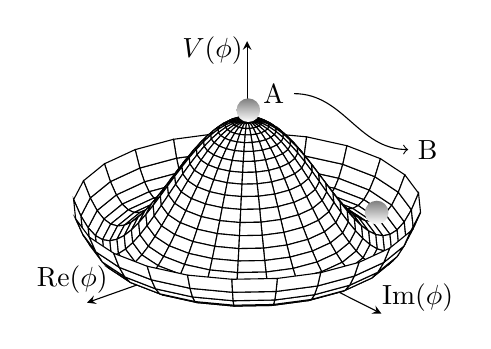
\begin{tikzpicture}
                    \begin{axis}[
                        axis lines=center,
                        view={140}{25},
                        axis equal,
                        domain=0:360,
                        y domain=0:1.25,
                        xmax=1.5,ymax=1.5,zmin=0,zmax=1.5,
                        x label style={at={(axis description cs:0.18,0.29)},anchor=north},
                        y label style={at={(axis description cs:0.82,0.25)},anchor=north},
                        z label style={at={(axis description cs:0.44,0.8)},anchor=north},
                        xlabel = $\mathrm{Re}(\phi)$,
                        ylabel=$\mathrm{Im}(\phi)$,
                        zlabel=$V(\phi)$,
                        ticks=none,
                        clip bounding box=upper bound
                        ]
                        \addplot3 [surf, shader=flat, draw=black, fill=white, z buffer=sort] ({sin(x)*y}, {cos(x)*y}, {(y^2-1)^2});
                    \end{axis}
                    \shade (3.47,3.5) circle [radius=0.15cm];
                    \shade (5.1,2.2) circle [radius=0.15cm];
                    \node[anchor=east] at (4.05,3.71) (text) {A};
                    \node[anchor=west] at (5.5,3.0) (description) {B};
                    \draw (description) edge[out=180,in=0,<-] (text);
                \end{tikzpicture}
                \caption{Higgs potential $V(\phi)$ with a minimum at $\phi^\dagger \phi = \frac{v^2}{2}$.}
                \label{fig:higgs_potential}
            \end{figure}
            When the Higgs field takes its VEV, the \(SU(2)_L \times U(1)_Y\) symmetry is spontaneously 
            broken down to \(U(1)_{\text{em}}\), the gauge symmetry of electromagnetism.
            Three of the four degrees of freedom in the Higgs doublet become the longitudinal 
            components of the W and Z bosons, giving them mass. 
            The remaining degree of freedom manifests as the physical Higgs boson.
        
            The masses of the W and Z bosons arise from the interaction between the gauge fields and the Higgs field.
            The charged W bosons (\(W^\pm\)) acquire mass through the term involving the Higgs VEV:
            \[
            (D_\mu \langle \phi \rangle)^\dagger (D_\mu \langle \phi \rangle).
            \]
            Expanding the covariant derivative:
            \[
            D_\mu \langle \phi \rangle = \left( \partial_\mu - i g \frac{\tau^a}{2} W_\mu^a - i g' \frac{Y}{2} B_\mu \right) \frac{1}{\sqrt{2}} \begin{pmatrix} 0 \\ v \end{pmatrix}.
            \]
            The term \(\frac{1}{2} g v W_\mu^1 - \frac{1}{2} g v W_\mu^2\) gives rise to the mass of the W bosons:
            \[
            M_W = \frac{gv}{2}.
            \]
            The neutral Z boson acquires mass similarly, but involves a mixture of \(W^3\) and \(B\):
            \[
            Z_\mu = \cos \theta_W W_\mu^3 - \sin \theta_W B_\mu,
            \]
            where \(\theta_W\) is the Weinberg angle. The mass of the Z boson is:
            \[
            M_Z = \frac{\sqrt{g^2 + g'^2} v}{2}.
            \]
            The photon remains massless because the corresponding combination of \(W^3\) and \(B\):
            \[
            A_\mu = \sin \theta_W W_\mu^3 + \cos \theta_W B_\mu,
            \]
            does not acquire a mass term from the Higgs mechanism.

        \subsubsection{Generation of fermion masses}
            The masses of the fermions (quarks and leptons) in the Standard Model 
            are generated through their interactions with the Higgs field. This 
            mechanism, known as the Yukawa interaction, couples the fermions to 
            the Higgs field, leading to mass terms once the Higgs field acquires 
            a VEV. 
            The Yukawa interactions describe the coupling between the Higgs field and
            the fermions. The relevant terms in the Lagrangian for a single generation 
            of quarks are:
            \[
            \mathcal{L}_{\text{Yukawa}} = -y_u \bar{Q}_L \tilde{\phi} u_R - y_d \bar{Q}_L \phi d_R + \text{h.c.}
            \]
            \(Q_L\) is the left-handed quark doublet:
            \[
            Q_L = \begin{pmatrix} u_L \\ d_L \end{pmatrix}.
            \]
            \(u_R\) and \(d_R\) are the right-handed up-type and down-type quark singlets, respectively.
            \(y_u\) and \(y_d\) are the Yukawa coupling constants for the up-type and down-type quarks, respectively.
            Recall the VEV of the Higgs field:
            \[
            \langle \phi \rangle = \frac{1}{\sqrt{2}} \begin{pmatrix} 0 \\ v \end{pmatrix}.
            \]
            Substituting the VEV of the Higgs field into the Yukawa Lagrangian, we obtain the mass terms for the quarks:
            \[
            \mathcal{L}_{\text{Yukawa}} = -y_u \bar{Q}_L \begin{pmatrix} 0 \\ \frac{v}{\sqrt{2}} \end{pmatrix} u_R - y_d \bar{Q}_L \begin{pmatrix} \frac{v}{\sqrt{2}} \\ 0 \end{pmatrix} d_R + \text{h.c.}
            \]
            This simplifies to:
            \[
            \mathcal{L}_{\text{Yukawa}} = -\frac{y_u v}{\sqrt{2}} \bar{u}_L u_R - \frac{y_d v}{\sqrt{2}} \bar{d}_L d_R + \text{h.c.}
            \]
            The terms \(\bar{u}_L u_R\) and \(\bar{d}_L d_R\) are Dirac mass terms for the up-type and down-type quarks, 
            respectively. Identifying the mass terms, we have:
            \[
            m_u = \frac{y_u v}{\sqrt{2}}, \quad m_d = \frac{y_d v}{\sqrt{2}}.
            \]
            Thus, the masses of the quarks are proportional to their respective Yukawa couplings.

            The generation of lepton masses follows a similar process, the Yukawa interactions for the leptons are given by:
            \[
            \mathcal{L}_{\text{Yukawa}} = -y_e \bar{L}_L \phi e_R + \text{h.c.}
            \]
            where \(L_L\) is the left-handed lepton doublet:
            \[
            L_L = \begin{pmatrix} \nu_{eL} \\ e_L \end{pmatrix}.
            \]
            where \(y_e\) is the Yukawa coupling constant for the electron.
            Substituting the VEV of the Higgs field into the Yukawa Lagrangian for leptons, we get:
            \[
            \mathcal{L}_{\text{Yukawa}} = -y_e \bar{L}_L \begin{pmatrix} 0 \\ \frac{v}{\sqrt{2}} \end{pmatrix} e_R + \text{h.c.}
            \]
            This simplifies to:
            \[
            \mathcal{L}_{\text{Yukawa}} = -\frac{y_e v}{\sqrt{2}} \bar{e}_L e_R + \text{h.c.}
            \]
            The term \(\bar{e}_L e_R\) is a Dirac mass term for the electron (or charged lepton), and the mass of the electron is:
            \[
            m_e = \frac{y_e v}{\sqrt{2}}.
            \]
            Therefore, the mass of the electron (or any charged lepton) is also proportional to its respective Yukawa coupling.
\section{A gravitational extension to the Standard Model}
        One potential extension for the SM to describe gravitation is proposed by Lisa Randall and Raman Sundrum~\cite{Graviton_theory},
        exploring the framework of a new higher-dimensional mechanism for solving the hierarchy problem~\cite{Arkani_Hamed_1998}.
        This model proposes a geometric solution to the hierarchy problem and predicts the existence of 
        Kaluza-Klein (KK) Graviton modes~\cite{Overduin_1997}. 
        Detailed explanations of technical aspects discussed briefly below can be found in ref.~\cite{Graviton_theory,Arkani_Hamed_1998,Overduin_1997}.
        The Randall-Sundrum (RS) model provides a geometric interpretation of the hierarchy 
        between the gravitational scale, \( M_P \sim 10^{18} \, \text{GeV} \), 
        and the weak scale, \( M_W \sim 10^2 \, \text{GeV} \). 
        In this model, the background geometry is a five-dimensional 
        Anti-de Sitter space (\( \text{AdS}_5 \)), characterised 
        by a constant negative curvature, and is truncated by two 
        four-dimensional Minkowski branes separated by a fixed distance~\cite{Arkani_Hamed_1998}.
        The model assumes that all relevant parameters arise naturally 
        from various powers of the five-dimensional fundamental scale, \( M_5 \sim M_P \).
        In the RS framework, the SM fields are confined to one of 
        the four-dimensional boundaries, commonly referred to as the 
        SM brane. The metric induced on this brane generates a 
        physical scale \( \Lambda_\pi \sim M_W \) from the 
        five-dimensional fundamental scale \( M_5 \), 
        achieved through an exponential geometric warp factor~\cite{Arkani_Hamed_1998}. 
        This warping effect eliminates the need to introduce 
        large hierarchies, as the exponential factor naturally 
        bridges the gap between the fundamental and electroweak scales.
        A key prediction of the RS model is the appearance of 
        spin-2 resonances, \( G^{(n)} \), which represent the 
        Kaluza-Klein (KK) excitations of the five-dimensional Graviton. 
        The masses and couplings of these resonances are determined 
        by the physical scale \( \Lambda_\pi \), making them potentially 
        significant for processes occurring at the weak scale.

        The RS model involves a 5D spacetime with the following metric:
        \[
        ds^2 = e^{-2kr_c|\phi|} \eta_{\mu\nu} dx^\mu dx^\nu - r_c^2 d\phi^2,
        \]
        where \( k \) is a scale of order the Planck scale. 
        \(\eta_{\mu\nu}\) is the 4D Minkowski metric. 
        \(\phi\) is the coordinate of the extra dimension, ranging from \(-\pi\) to \(\pi\).
        In this space, four-dimensional mass scales are related to five-dimensional mass parameters and the $e^{-2kr_c|\phi|}$, the warp factor.
        In the RS model, the Graviton field \(h_{\mu\nu}(x, \phi)\) can be expanded in terms of KK modes:
        \[
        h_{\mu\nu}(x, \phi) = \sum_{n=0}^{\infty} h_{\mu\nu}^{(n)}(x) \frac{e^{-2kr_c|\phi|}\chi^{(n)}(\phi)}{\sqrt{r_c}},
        \]
        where \(h_{\mu\nu}^{(n)}(x)\) are the 4D Graviton modes. 
        \(\chi^{(n)}(\phi)\) are the wave-functions of the KK modes that only depend on the extra dimension, \(\phi\) and \(r_c\).
        \(\chi^{(n)}(\phi)\) can be written as:
        \[
            \chi^{(n)}(\phi) \approx \frac{e^{2kr_c|\phi|}}{N_n}J_2\left(\frac{m_n}{k} e^{-kr_c|\phi|}\right),
        \]
        where $J_l$ is the $l^{th}$ order Bessel function. $m_n$ is the mass of the $n^{th}$ KK Graviton,
        and $N_n$ is a normalisation factor, given by:
        \[
            N_n \approx \frac{e^{kr_c\pi}}{\sqrt{kr_c}} J_2(x_n).
        \]
        The effective 4D Lagrangian for the interaction between KK Gravitons and the SM fields is:
        \[
        \mathcal{L}_{\text{eff}} = -[\frac{1}{M_P} h_{\mu\nu}^{(0)} T^{\mu\nu} - \frac{1}{\Lambda_\pi} \sum_{n=1}^{\infty} h_{\mu\nu}^{(n)}] T^{\mu\nu},
        \]
        where \(T^{\mu\nu}\) is the energy-momentum tensor of the SM fields and \(\Lambda_\pi = M_P e^{-kr_c\pi}\) is the effective scale on the TeV brane.
        Studies of the RS model have focused on the $\mathcal{L}_{\text{eff}}$ interaction. These interactions are only suppressed by $\Lambda_\pi$.
        In this thesis, we focus on the Graviton coupling to the SM Higgs boson, with low-TeV masses, the production cross section of the Higgs boson pairs 
        from the KK Graviton resonances is predicted to be significant at the current energy frontier.
        The 5D action, which describes gravity in the RS model, is:
        \[
        S_G = 2M_5^3 \int d^5x \sqrt{-G} R_5,
        \]
        where \(M_5\) is the 5D Planck scale, \(G\) is the determinant of the 5D metric \(G_{MN}\), and \(R_5\) is a 5D scalar.
        Interactions also occur between the \( G^{(n)} \) resonances arising from the \( S_G \). 
        The leading term in this self-coupling, in terms of powers of \( M_5^{-1} \), 
        is the triple Graviton vertex. 
        In four dimensions, this implies that the coupling between three 
        KK Gravitons \( \{ G^{(l)}, G^{(m)}, G^{(n)} \} \), 
        is governed by powers of \( \Lambda_\pi^{-1} \), 
        making it the dominant interaction within the KK Graviton sector.
    
\section{Modelling proton-proton collisions in particle physics}
    Proton-proton collisions, such as those studied at the Large Hadron Collider, 
    are complex processes modelled in several stages: parton distribution functions, hard scattering,
    parton showering, hadronisation, and underlying events. A typical collision
    is shown in Figure~\ref{fig:pp_collision}.

    \begin{figure}[htbp]
        \centering
        \includegraphics[width=1.0\textwidth]{Raster/pp-evt.pdf}
        \caption{
            Sketch of how a hadron collision is modelled. 
            In particular, one can notice the initial states, hard scattering, parton shower, hadronisation and the so-called underlying event. 
            From INFN web-page~\cite{pp_event_sketch}.
        }
        \label{fig:pp_collision}
    \end{figure}

    \subsection{Parton Distribution Functions (PDFs)}
        Protons are not fundamental particles; they are bound states of $uud$ quarks and gluons, collectively known as partons. 
        The PDF, \( f_i(x, Q^2) \), gives the probability density for finding a parton of type \( i \) (where \( i \) could 
        be \( u, d, s, c, t, b \) for quarks and \( g \) for gluons) with a momentum fraction \( x \) at a scale \( Q^2 \):
        \[
        f_i(x, Q^2) = x q_i(x, Q^2),
        \]
        where \( q_i(x, Q^2) \) is the number density of partons of type \( i \).
        The PDFs are extracted from experimental data and theoretical calculations 
        and are essential for predicting initial states in collisions.
        The Dokshitzer-Gribov-Lipatov-Altarelli-Parisi (DGLAP) equations describe how PDFs evolve with the energy scale \( Q^2 \):
        \[
        \frac{\partial f_i(x, Q^2)}{\partial \ln Q^2} = \sum_j \int_x^1 \frac{dy}{y} P_{ij}\left(\frac{x}{y}, \alpha_s(Q^2)\right) f_j(y, Q^2),
        \]
        where \( P_{ij}(z, \alpha_s) \) are the splitting functions, which describe the probability of a parton
        \( j \) splitting into a parton \( i \) with a fraction \( z \) of the momentum. And \( \alpha_s(Q^2) \) 
        is the strong coupling constant.

        The DGLAP equations can be written in a convolution form, showing the relationship between PDFs and splitting functions:
        \[
        \frac{\partial f_i(x, Q^2)}{\partial \ln Q^2} = \sum_j \left( P_{ij} \otimes f_j \right)(x, Q^2),
        \]
        where the convolution is defined as:
        \[
        \left( P_{ij} \otimes f_j \right)(x, Q^2) = \int_x^1 \frac{dy}{y} P_{ij}\left(\frac{x}{y}, \alpha_s(Q^2)\right) f_j(y, Q^2).
        \]
        In a proton-proton collision, the differential cross-section for a process \( pp \rightarrow X \) 
        involving partons \( i \) and \( j \) can be written as:
        \[
        d\sigma = \sum_{i,j} \int dx_1 dx_2 f_i(x_1, Q^2) f_j(x_2, Q^2) d\hat{\sigma}_{ij \rightarrow X},
        \]
        where \( d\hat{\sigma}_{ij \rightarrow X} \) is the partonic cross-section for the subprocess \( ij \rightarrow X \).
        One of the most widely used PDF sets are produced by the NNPDF (NN-based Parton Distribution Function) collaboration, 
        which uses neural networks to parameterise PDFs~\cite{Ball_2022}. 
        The NNPDF4.0NNLO sets are shown in Figure~\ref{fig:NNPDF40N2LO} for the PDFs at $Q = 3.2~\GeV$ and $Q = 100~\GeV$.
        This set approximates the PDFs at next-to-next-to-leading order (NNLO) precision.
        \begin{figure}[htbp]
            \centering
            \includegraphics[width=1.0\textwidth]{Raster/nnpdf4.0.png}
            \caption{
                The NNPDF4.0NNLO parton distribution functions at $Q = 3.2~\GeV$ and $Q = 100~\GeV$~\cite{Ball_2022}.
            }
            \label{fig:NNPDF40N2LO}
        \end{figure}
        The latest NNPDF releases incorporate QED corrections, marking a significant step forward~\cite{thennpdfcollaboration2024photonsprotonimplicationslhc}. 
        They account for the photon parton distribution function, which, although a small correction, impacts the momentum fraction carried by the gluon. 
        The collaboration has made steps towards the next order of precision, approximate N3LO (Next-to-Next-to-Next-to-Leading Order). 
        The N3LO PDFs includes higher-order corrections in the PDFs, the predictions improves.
        The N3LO PDFs are consistent with NNLO results within uncertainties~\cite{thennpdfcollaboration2024pathn3lopartondistributions}.
        A significant milestone achieved by the NNPDF collaboration is the evidence for intrinsic charm quarks within the proton. 
        The intrinsic charm component was disentangled from charm-anticharm pairs arising from high-energy radiation, with a significance of three standard deviations~\cite{thennpdfcollaboration2022charmintrinsic}.

    \subsection{Parton shower, hadronisation, and underlying event}
        After the initial hard scatter, the high-energy partons undergo a cascade of emissions, producing more partons. 
        This process, described by perturbative QCD, includes both initial-state radiation (before the collision) and 
        final-state radiation (after the collision). The parton shower accounts for the sequential splitting of partons, 
        resulting in a multitude of lower-energy partons. 
        As partons cannot exist in isolation due to colour confinement, they must transform into colour-neutral hadrons. 
        hadronisation is a non-perturbative process where partons combine to form hadrons (e.g., pions, protons). 
        Two common models used to describe hadronisation are the Lund string model and cluster fragmentation. This 
        process occurs over a very short distance and time scale, effectively turning the showered partons into detectable 
        particles.
        Besides the primary hard scatter, other interactions occur in the collision, collectively known as the underlying event. 
        This includes additional soft parton interactions, beam-beam remnants (particles that do not participate in the hard scatter).
        The underlying event contributes to the overall activity observed in a collision 
        and must be accurately modelled to distinguish the signal from the background.
        Together, these processes transform the initial high-energy partons into a rich final state of hadrons that experimental 
        detectors can observe and analyse. Understanding each stage is crucial for accurate simulation and interpretation of collider data.